\documentclass[10pt,a4paper]{article}
\usepackage{graphicx}
\usepackage{hyperref}
\usepackage{natbib}
\usepackage{booktabs}
\usepackage{makeidx}
\usepackage{tgpagella}
\usepackage[T1]{fontenc}

\hypersetup{
    colorlinks=true,       % false: boxed links; true: colored links
    linkcolor=black,          % color of internal links
    citecolor=black,        % color of links to bibliography
    filecolor=magenta,      % color of file links
    urlcolor=black           % color of external links
}

\title{Technical patterns for linking organizations with X-Road}
\author{Estonian Information System Authority}

\begin{document}

\maketitle
\clearpage
\setcounter{tocdepth}{2}
\tableofcontents
\clearpage

\section{Background}
\subsection{Introduction}
This is document seeks to collect descriptions of architectural patterns that make sense to be used around x-road. The patterns identified are listed in \ref{tab:dir}, but currently only two of them have been described in detail.

While all the patterns are usable, no tool is usable for every purpose. Therefore, the patterns are each classified along a set of dimensions allowing for easier navigation and comprehension. The dimensions are defined as follows:
\begin{description}
	\item[Doc\textbackslash Data\textbackslash Service] All of the patterns are particularly suitable for either transmitting documents, data or providing a service. If a patterns is marked as suitable, this means it works well in a given setting and a missing mark means the pattern is not really suitable for a purpose. \index{Document}
	\item[Volume] The volume property denotes the amount of requests a particular pattern is useful for. This is not about absolute numbers but rather relative ones. A pattern marked with \"M\" is suitable for smaller volumes than the one with a \"L\" marking
	\item[Doc direction] Not all patterns are symmetrical in nature. If a document is passed in a transaction, it can move up, down or both ways of the stream. This column indicates, whether the pattern works well for up-stream documents (U), downstream documents (D) or can handle both directions equally well (B). The patterns not suitable for documents are not marked in this column
	 \item[Availability] The systems being integrated might have different availability requirements. If they do, it is important to make sure the availability of one system is not compromised by the availability of the other. This dimension indicates, how the availability of the system in question compares with the one of the integrated system
\end{description}

In the document, Alice is used to denote the organisation implementing the pattern whether as a consumer or provider with Bob referring to the other side of the interaction.

\begin{table}
	\begin{center}
		\begin{tabular}{p{.6cm}p{3.4cm}p{.8cm}p{.8cm}p{.8cm}p{.8cm}p{1.2cm}p{1.2cm}}
		\toprule
ID & Pattern & Doc & Data & Service & Volume & Doc direction & Availability \\
\midrule
1 & Straight up xRoad &  & X &  & S &   & eq \\
2 & Consumer pool & X & X & X & M & D & $\geq$ \\
3 & Adapterserver &  & X &  & S &   & eq \\
4 & DVK & X &  &  & M & B & > \\
5 & Async xRoad provider/consumer & X & X & X & L & U/D & $\leq$ \\
7 & Async xRoad SS & X & X &  & M & B & eq \\
8 & Gateway to xRoad &  & X & X & L &   & $\geq$ \\
9 & Reconciliator & X & X & X & XL & B & $\leq$ \\
10 & Dead Letter & X & X &  & XL & U & > \\
11 & Document store & X & X &  & L & U & > \\
12 & Replica &  & X &  & XL &   & $\gg$ \\
13 & Read-through cache &  & X &  & XL &   & $\gg$ \\
14 & Pub-sub &  & X &  & L &  & < \\
15 & Delivery at least once & X & X & & XL & U/D & $\geq$ \\
16 & Aggregated middleware & X & X & X & XL & U/D & eq \\
\bottomrule
		\end{tabular}
		\caption{Summary of the patterns}
		\label{tab:dir}
	\end{center}
\end{table}

\section{Asynchronous x-road provider/consumer}
\label{sec:p:5}
\subsection{Overview}
It is usually undesirable that the dynamic complexity \index{Dynamic complexity!leakage} of Bob leaks over the system boundary to Alice or vice versa. To prevent this from happening, two buffers are used to separate Alice from the rest of the world. There is a request adapter that, upon receiving an incoming request, validates it for syntactic error and, upon success, posts a message to the requests queue\index{Queue}. If that succeeds, a "message understood, received and persisted" response to Bob can be sent immediately. On the other end of the queue, there is a worker that consumes the messages and actually provides the necessary services using the information system. The response to the request is then posted to the response queue from where it is picked up by the response worker who sends it back to Bob via another xRoad service. All active components, the request adapter, response worker and the worker, can be multiplied to provide better scalability. The pattern is depicted on figure \ref{fig:p:5}

\begin{figure}[htp]
	\begin{center}
		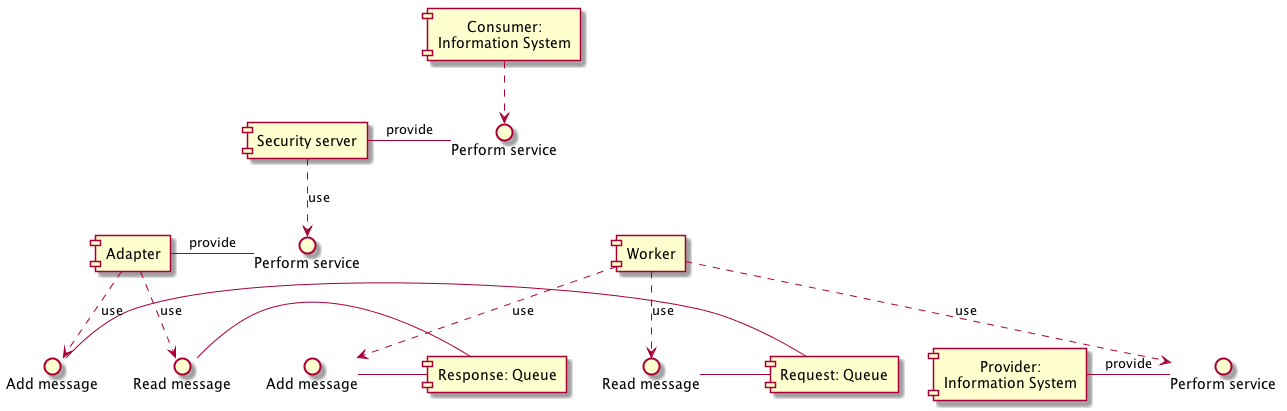
\includegraphics[width=1\textwidth]{5_comp.png}
		\caption{Asynchronous xRoad provider/consumer pattern}
		\label{fig:p:5}
	\end{center}
\end{figure}

\subsection{Summary}
\begin{description}
	\item[Paradigm orientation] The pattern is suitable for documents, data and service
	\item[Volume preference] Although message queueing and transformation adds overhead, the pattern is still usable for large request volumes
	\item[Direction] The pattern is intended for consuming services but, when reversed, can be used for provision equally well
	\item[Availability] The pattern is suitable for situations where the availability requirements of the Alice side are much higher than on Bob's side
\end{description}

\subsection{Details}
The function of components depicted on figure \ref{fig:p:5} is as follows.
The worker reads messages from the queue and forwards them to the information system for processing. The latter process might either be asynchronous or synchronous. In either case, the worker composes a response message and posts it to the response queue. The worker serves an important function as the guardian of the information system by not submitting more messages than is agreed upon. In case multiple worker instances are present, two synchronisation mechanisms must be present: one to prevent maximum throughput limits being breached and another one (should message order be important) assuring messages are forwarded in order. It is important to note that the one to one relationship between request and response messages is not necessary: a single request might generate multiple responses and the other way around. The worker also acts as a translator (todo: insert pattern reference here) by transforming the message format and semantics of the external interface to a format that is suitable for the information system. 

The adapter compiles the request message and implements the service exposed to the third party. It is not subject to throttling and processes requests at a rate they come in. The adapter might be implemented in three fundamental ways. Firstly, it might respond immediately with a "message received, understood and persisted" message. In this case, any further response from the information system is either meaningless (e.g. the request is for data upload) or delivered by some other means. The first implementation option makes the adapter  stateless and thus easily scalable. Secondly, the adapter might wait for the response message to arrive before responding and hide the asynchronous nature of the implementation entirely. In the latter case, the adapter becomes stateful and thus harder to scale. Also, it must implement the logic for providing error messages in case of delayed responses, deal with multiple request issues. Finally, the adapter might take responsibility for delivering the response messages to Bob. Figure \ref{fig:p:5:async} depicts all three implementation options as a sequence diagram.

Regardless of other details, the adapter and worker must implement an identical set of message formats for request response. For the message formats, it is critical that there is a way to correlate request and response messages with each other and with the incoming request from Bob. One of the simplest ways to achieve this is supplying messages with unique identifiers and maintaining a metadata section with the transaction log referencing these. This being is the only dependency between the worker and the adapter highlights the key advantage of this pattern: separation of business logic from the interface logic. Adapter takes care of the latter while worker encapsulates the former.

\begin{figure}[htp]
	\begin{center}
		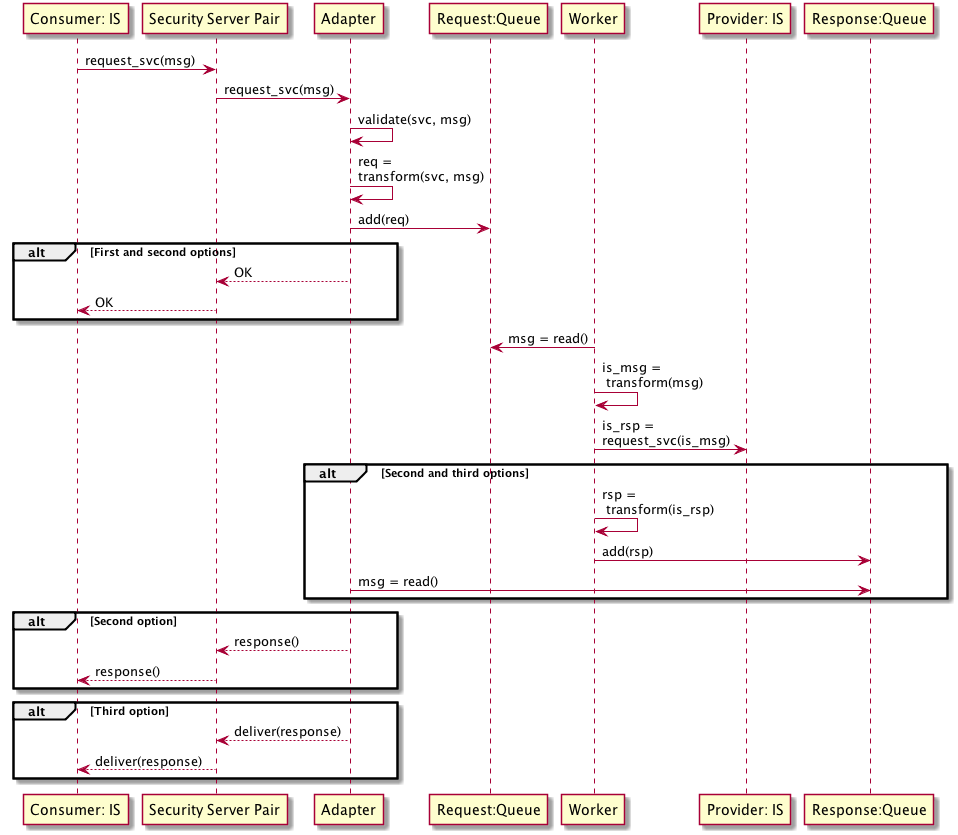
\includegraphics[width=.85\textwidth]{5_seq.png}
		\caption{Sequence diagram of the asynchronous service provider}
		\label{fig:p:5:async}
	\end{center}
\end{figure}

As depicted on figure \ref{fig:p:5:async}, processing of a request is comprised of following steps:

\begin{enumerate}
	\item A request for service is received from the security server
	\item Adapter validates the message against an agreed-upon syntax. At this point, the amount of processing is minimised and only formal validation is conducted. For example, the adapter might verify that an address field is filled but does not confirm if the address in the field is indeed valid.
	\item Adapter transforms the request into a format that can be understood by the worker adding the necessary metadata and, if necessary, generating message identifiers
	\item The message is added to the request queue
	\item In case the response does not carry meaning or will be delivered later, a message is sent to the security server confirming message delivery
	\item The worker reads a message from the request queue 
	\item The message is transformed to a format the information system understands by striping (but not discarding!) headers. It is likely that at this point a protocol transformation also takes place by, for example, making a request towards a CORBA\footnote{CORBA stands for Common Object Request. It is an older remote command invocation protocol mainly used in enterprise-class solutions} server. 
	\item In case the response from the information system is meaningful, it is transformed into a message the adapter can understand and posted to the response queue
	\item The adapter server reads a message from the response queue and matches it to a request so it can be delivered
	\item In case the customer is still waiting, the response is delivered
	\item If the customer has left, the adapter server takes active measures to deliver the message. In this case, the original message from the security server must contain some call-back mechanism so the adapter knows where a particular message is to be delivered 
\end{enumerate}

\subsection{SWOT}
\subsubsection{Strengths}
	\begin{itemize}
		\item The pattern effectively prevents dynamic complexity leakage across organisational boundaries. While both the worker and the external customer agree to adhere to a certain behaviour, only the worker can be guaranteed to do so. In case the requests come in faster than the information system can handle, the request queue starts growing. Once the situation is reversed, the queue shrinks again. This independence allows for simpler service level agreements with the partner. Also, there is now flexibility around what that behaviour is at a given moment permitting to compliance with service windows and the like. 
		\item The timeouts are under control. In any integration scenario, proper handling of timeouts in an explicit manner is of paramount importance as a raw timeout is an uncertain event. There is no knowledge about what exactly happened and on what level the timeout actually occurred. Did the message get delivered and processed with the network timing out during response delivery or was the request not received because of network issues? In a direct integration scenario, the resources of the processing system are busy processing incoming requests and its ability to produce an error log or a meaningful error message is limited. This also means transactional integrity is much better preserved as the state of the exchange is know with much higher probability to both parties 
		\item Bob can be released rapidly. In case the response is not meaningful or the reconciliator pattern is used (see section \ref{sec:p:9}) Bob can rapidly be confirmed that the message has been correctly received releasing its resources. Otherwise Bob might be waiting until the message is fully processed, ready to receive a negative response and act upon it. Such waiting can very resource-intensive for high-throughput use cases. 
		\item Transactional integrity is rather well preseverd. If the security server communicated directly with the information system
	\end{itemize}

\subsubsection{Weaknesses}
	\begin{itemize}
		\item The pattern is developmentally complex. Compared to the standard model, there are more moving parts and protocols to agree upon, specify, build and change. Therefore, its upsides in terms of more sensible behaviour towards Bob and better resilience towards his possibly erratic manners must be carefully considered.
		\item The pattern is operationally complex containing many more elements to be deployed and maintained. See section \ref{sec:p:6:ops} for a more detailed discussion of this
		\item Business process complexity for handling issues. This is actually a strength in disguise as in case of the standard model, there are many situations where a failed interaction leaves no meaningful traces. The asynchronous pattern however surfaces such issues at either at the worker  (what if Bob was told everything was fine but the information system fails to process the request?) or at the adapter (I have a response message but Bob has dropped the connection. What do I do with the response?). Figuring out what the correct behaviour is might not be trivial but typically the issues are too glaring for developers to simply ignore.
	\end{itemize}

\subsubsection{Opportunities}
	\begin{itemize}
		\item Dynamic scalability. When the standard approach is used, there is no way to react to a rapid increase of load. In case of this pattern, however, the increase of the request queue can be detected. Should that be the case, resources might be added either to information system, the worker or both, so increased load can be handled without architectural changes. Alternatively, the adapter server might gracefully reject some requests
		\item Multi-step processing. Since the interaction with the partner is separated from actually processing the message, it is possible to make the processing consist of multiple steps. For example, one might add a step to enrich the incoming message with additional data. TODO: insert pattern reference. Also, the same request can be utilised for multiple purposes. For example, it can be used for both the formal processing by the information system as well as producing statistics. 
	\end{itemize}

\subsubsection{Threats}
The main threat in case of this pattern is invalid communication of response code. That threat is, of course, always present but here the palette of possible conditions is much wider making for a more complex semantic space. In case of the standard model, a "OK" response has a definitive meaning of the message being received and processed. Here, "OK" might mean that the message has been received, validated and persisted but subsequently lost due to a failure by the queue provider. Also the boundary between structural and process correctness of messages can be hazy (does the validity of an address mean it is a valid string, that it is a validly formatted address or that the address actually exists in a database somewhere). 

To counter this threat, the semantics of response code as well as the entire behaviour of the interface must be very well documented and the test cases in use ought to test for the semantic boundaries described.

\subsection{Operational considerations}
\label{sec:p:6:ops}
As mentioned before, one of the weaknesses of the asynchronous service provider pattern is its operational complexity. In addition to having more moving parts, it slightly alters the notion of performance monitoring. Since the components are not rigidly dependent on each other, they can commonly work at their optimal performance point. Thus it might be difficult to determine, if system performance is adequate in relation to incoming load. Commonly, server resources like CPU, memory and threads are monitored\index{Monitoring} for this end, but this pattern is designed to keep these parameters stable. Instead, queue status should be monitored: spikes in incoming (or, outgoing) queue lengths indicate whether or not demand is handled adequately. In general, a more complex system can behave in more complex ways and thus properly thought out monitoring is important for this pattern.

In case the demand can not indeed be satisfied, the adapter should be able to gracefully reject incoming requests. This can be done in multiple ways. Assuming the client is adequately capable, one might respond with HTTP 503 response code and utilise the \texttt{Retry-After} header as described in \cite{RFC2616}. An other, possibly more transparent, option is to modify the API provided to contain this sort of rejection.

Another operational consideration for this pattern is the availability of the queues. Since they play a key role in system availability, they should have a very robust availability model preventing data loss. For these purposes, it is probably a good idea to share the queue provider between different systems so headroom can be pooled.

Finally, this patterns can grow operationally more complex if more than one instance of the Adapter component are present. With one adapter, it can be guaranteed that the same component that maintains a connection to the customer via the SecurityServer also receives a response message. With multiple adapters this is no longer the case. For multiple Adapters to work, the messages passed must contain a reference to the adapter as well as the originating connection and the queue implementation must support ''peeking'' i.e. looking at a message and returning it to the queue untouched.
 
\section{Reconciliator}
\label{sec:p:9}
\index{Reconciliator}
\subsection{Overview}
In case of high-volume or high-importance interaction, it is often important to make sure both sides have the same understanding of what has happened and detect errors. The errors might be caused by technical issues in the communication stack, by failures of either party or because of logical discrepancies stemming, for example, from different interpretations of the response codes. Detection and automated recovery of such errors is especially important in financial settings where, for example, books might be closed daily. For this purpose, a detailed log of all interactions is kept and a special subsystem frequently attempts to reconcile that log with Bob. For simple cases, both Alice and Bob might expose an interface for just comparing the sum of all transactions processed but in more complex settings detailed information like a list of all package IDs might be exchanged. The pattern is depicted on figure \ref{fig:p:9}.
\begin{figure}[htp]
	\begin{center}
		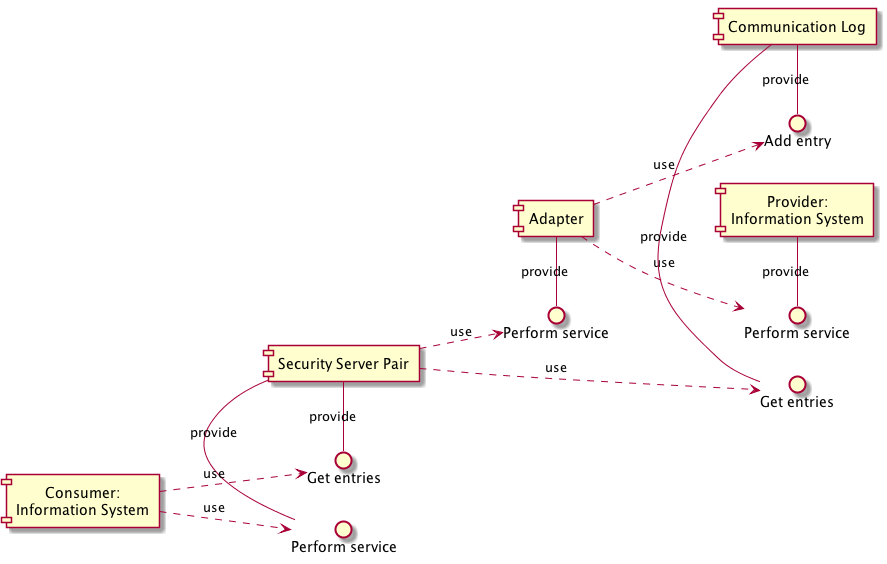
\includegraphics[width=1\textwidth]{9_comp.png}
		\caption{Reconciliator pattern}
		\label{fig:p:9}
	\end{center}
\end{figure}

\subsection{Summary}
\begin{description}
	\item[Paradigm orientation] The pattern is suitable for documents, data and service
	\item[Volume preference] Unless a very noisy communication channel is used, the pattern only becomes useful under very large request volumes
	\item[Direction] The pattern is agnostic towards service direction and could be used by both parties simultaneously
	\item[Availability] The pattern is suitable for situations where the availability requirements of the Alice side are higher than on Bob's side
\end{description}

\subsection{Details}
Figure \ref{fig:p:9} contains the component diagram of the reconciliator pattern. The adapter component is responsible for intermediating a service from the security server to the information system. When doing that, it logs the interaction along with its outcome in the communication log. Note, that this creates a problem known as multi-phase commit\index{multi-phase commit}: we must make sure that the service outcome in the information system and the log are the same. While this is the same fundamental problem the pattern is meant to solve, both parties of the issue are now local and one of them, the communication log, can be very simple. Having reduced the problem to a well-known one, we leave the detailed solution to the reader as an exercise. The communication log exposes an additional interface to the security server allowing for access to the stored log events. These can be accessed then by the information system on Bob's side so system states can be compared. The event log might be detailed listing all logs with outcomes, might just contain failed interactions or just consist of aggregate results like sums. To limit the potential size and complexity of the reports, it is recommended that a maximum reconciliation horizon is agreed upon between parties.

The pattern can be implemented as two mirrored instances allowing for both parties to request for the state of the other. Although it is preferable the reconciliation to be automated, the pattern does not enforce it and the discrepancies found might be routed to a human agent for resolution.

\subsection{SWOT}
\subsubsection{Strengths}
	\begin{itemize}
 		\item Transactional integrity. The reconciliator pattern allows for both parties to ensure the information systems of all parties correctly reflect their logical business relationship  
		\item Operational flexibility. If a reconciliator is in place, the operational requirements between the parties drop significantly. Instead of having to implement correct recovery procedures for each error condition individually, it can now be assumed the reconciliator will transfer any messages dropped, for example, because of server restarts. Also, recovery from a data loss becomes a matter of generating a suitable report at the end of the reconciliation period
		\item Easy recovery from information system errors. In addition to interface errors, the pattern allows to recover from both technical and logical failures of the information system
		\item Robust business processes. Implementation of the reconciliator explicitly surfaces business process decisions around failure recovery. A more robust business process results. 
	\end{itemize}
	
\subsubsection{Weaknesses}	
	 	\begin{itemize}
			\item Higher complexity. In addition to the interfaces providing direct business value, the organisation must provide another interface along with everything that goes with it (documentation, operations, maintenance, testing etc.). Also, the solution to the local multi-phase commit\index{multi-phase commit} is not necessarily trivial
			\item Restrictions to the information system. In case a discrepancy is discovered between the states of the systems, the information system must allow for these to be rectified. For example, in case of financial systems, the reconciliation must take place before the common change-of-day\index{change-of-day} procedures or both systems must allow for changes in already closed books. 
			\item Relationships with the business process. The business process, in order to account for reconciliation, must take into account system failure making it more robust but at the same time requiring it to cross the usual competence boundaries between different responsibility areas
		\end{itemize}

\subsubsection{Opportunities}	
	 	\begin{itemize}
			\item Business meaning. Although the reconciliator is meant as a technical tool for (semi) automatic system reconciliation, it can be used to convey business meaning. For example, in addition to technical information, useful statistics, SLA\footnote{Service Level Agreement\index{SLA}. An agreement between two parties about the exact levels of services provided} reports. 
		\end{itemize}
\subsubsection{Threats}	
	 	\begin{itemize}
			\item Large volumes of data. In case large amounts of messages are exchanged, a naive reconciliation implementation can be resource-consuming for example, if a list of all messages exchanged is attempted to be transmitted. In order to prevent this, the semantics and structure of the report must be designed to work for all scenario (complete data loss on one side, for example) and message volumes
		\end{itemize}

\subsection{Operational considerations}
Form the operational perspective, the pattern offers few specific challenges. Although it is designed for easy recovery from system failures, excessive reliance on its abilities can cause of domino effect where a voluminous reconciliation report causes one of the systems to under-perform leading to more failed messages and more need for reconciliation. Also, the message log and information system must operationally be thought of as a logical entity, i.e. they should be backed up and recovered in a way that does not compromise their synchronicity. 

Since a two-phase commit problem now exists between an information system and the communication log, these two should be deployed in a way that minimises network uncertainty. Ideally, a shared transactional context might be used but shared hardware also provides some assurance. 

In terms of monitoring, the communication log is meant to potentially be able to recover from data loss spanning the entire life time of the system. For large and old systems, this might lead to unreasonable storage requirements. Thus it is recommended that the reconciliation horizon is agreed upon and enforced. 

\section{Read-through cache}
\label{sec:p:13}
\subsection{Overview}
\subsection{Summary}
Sometimes Alice does not need all of the data from Bob but would like to get rapid and independent answers to requests. In that case, Alice can implement a stub service that responds to all queries based on locally stored data or, if that is missing, executes a query towards Bob and caches the result. It might be that both options are used: while a local copy is served for speed, the cache is updated by requesting fresh information from Bob. The pattern is depicted on figure \ref{fig:p:13}.

\begin{figure}[htp]
	\begin{center}
		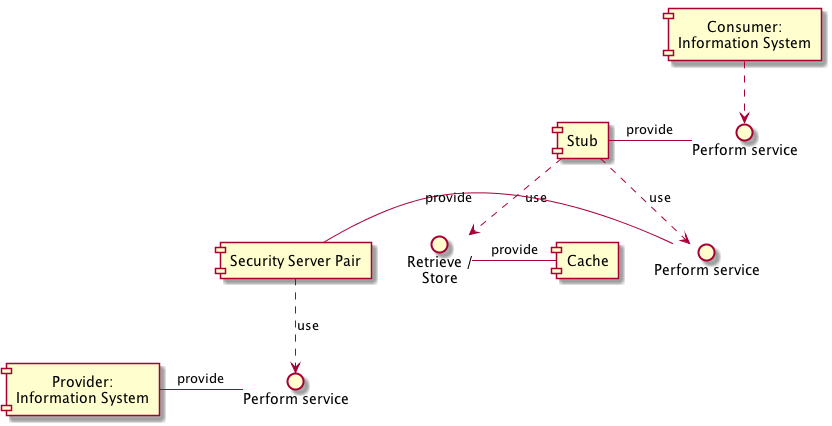
\includegraphics[width=1\textwidth]{13_comp.png}
		\caption{Read-through cache pattern}
		\label{fig:p:13}
	\end{center}
\end{figure}

\subsection{Details}
\subsection{SWOT}
\subsubsection{Strengths}
	\begin{itemize}
 		\item strength  
	\end{itemize}
	
\subsubsection{Weaknesses}	
	 	\begin{itemize}
			\item Weakness
		\end{itemize}

\subsubsection{Opportunities}	
	 	\begin{itemize}
			\item Opportunity
		\end{itemize}
\subsubsection{Threats}	
	 	\begin{itemize}
			\item threat
		\end{itemize}

\subsection{Operational considerations}

\clearpage

\bibliographystyle{plain}
\bibliography{xroad_distilled} 

\end{document}
